\subsection{Área de estudo e dados disponíveis}
O estudo foi realizado na região de São Paulo onde está localizado a bacia hidrográfica do Rio Tamanduateí (Figura 1). Esta bacia possui uma área de \(323km^2\) e se estende até as bacia hidrográficas do Rio Pinheiro, Rio Guaió, Rio Aricanduva e Córrego de Tapuapé. Nesta região, foi analisado a partir de um pluviômetro um raio espacial de \(2000m\) que abrange as regiões de alagamentos, tweets georrefenciados e a célula de radar.
\begin{figure}[H]
    \centering
    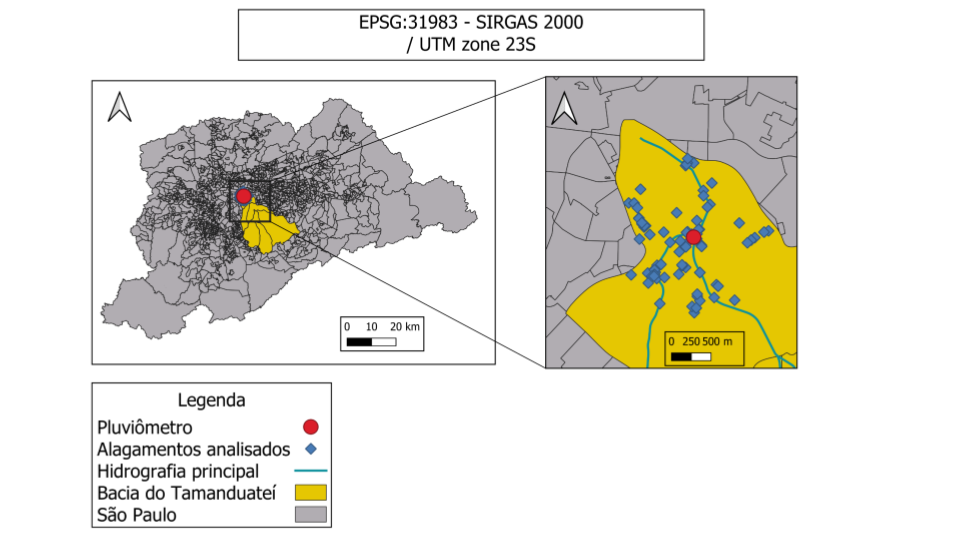
\includegraphics[scale=0.5]{imagens/ic_att.png}
    \caption{Área de estudo }
    \label{fig:my_label}
\end{figure}

\par Os dados da rede social Twitter foram extraídas através da API (\textit{Application Programming Interface}). Os dados pluviométricos são coletados do pluviômetro 833A, pertencente ao Centro Nacional e Alertas e Desastres Naturais (CEMADEN), estes dados podem ser encontrados no próprio site da instituição.  
\par A série histórica de alagamentos na área de estudo, foram concebidas por um dos integrantes da pesquisa. Os dados metereológicos foram extraídos por estações pertencentes ao CEMADEN, o equipamento está localizado na cidade de São Roque - SP e atualmente está em operação pelo Departamento de Controle do Espaço Aéreo (DECEA). Esse radar tem alcance de 250 km, cobrindo toda a região metropolitana de São Paulo. O produto de radar usado para o CAPPI (Constant Altitude Plan Position Indicator) na altura de 3 km. Este produto possui uma resolução espacial de aproximadamente 1 km e uma resolução temporal de 10 minutos. Para a conversão da refletividade (dBZ) em taxa de separação (mm / h) foi utilizado em relação a Marshall-Palmer \cite{marshall1948mc}) e a seguir os dados foram acumulados por dia. 
\subsection{Ferramentas }
A análise e aplicação do projeto será realizada de maneira geral com a ferramenta \textit{Python}. Para a manipulação, filtragem e tratamento dos dados será utilizada a biblioteca \textit{Pandas}, já a análise gráfica com \textit{Matplotlib} e \textit{Seaborn}. 
\par A aplicação de testes estatísticos na série de dados será usado \textit{Scipy} e \textit{Numpy}, para os modelos de apredizagem supracitados, a biblioteca específica para aprendizado de máquina denominado \textit{Scikit-learn}. Por fim, algumas filtrações no banco de dados de alagamentos será realizada com ferramentas de geoprocessamento do software \textit{QGIS}. 


\subsection{Proposta de algoritmo para definição do modelo}
A concepção inicial deste trabalho é analisar as séries temporais  dos alagamentos, tweets, pluviômetro e radar, para definir quais são o melhor conjuntos de parâmetros em dias de alagamentos, associando-se ao número mínimo necessário de tweets para emissão de um alerta. 
\par A série temporal analisada compreende os três primeiros meses do ano de 2019. Para a base de dados dos tweets, o processamento consiste no recorte temporal e filtração do tweets com base na lista de palavras associadas ao contexto metereológico e hidrológico. Esta lista de palavra basea-se no trabalho de \cite{de2021effect}. 
\par Com base na estrutura (Figura 2), será registrado em único arquivo, na mesma série temporal, o número de tweets filtrados, os valores de precipitação do radar e o pluviomêtro, e se houve alagamentos no dias analisados. Este dados processados em um único arquivo, possibilitarão a submissão nos modelos de aprendizados propostos, dividindo-se em base de dados para teste e treinamento.  
\begin{figure}[H]
    \centering
    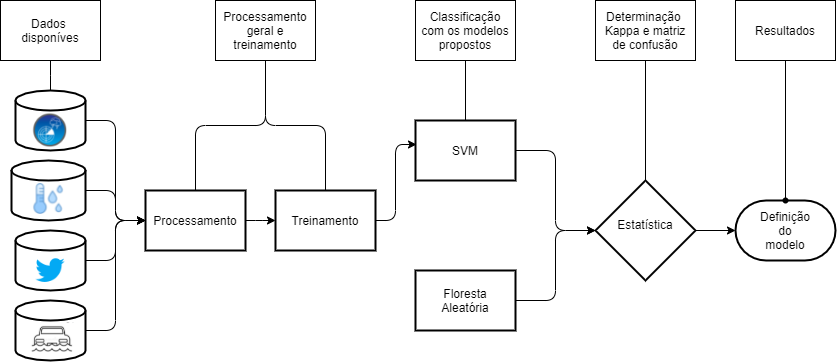
\includegraphics[scale=0.6]{imagens/att2.drawio.png}
    \caption{Metodologia}
    \label{fig:my_label}
\end{figure}
\par Como a classificação binária consiste em dias de alagamento e não alagamento, a acurácia será medida a partir da base de dados de teste. Após o treinamento nos modelo SVM e Floresta Aleatória e Redes Neurais, serão analisadas a acurácia através da validação cruzada e subsequentemente testes estatísticos como ANOVA e coeficiente Kappa, determinando-se assim, o algoritmo que possui maior potencial para o desenvolvimento de um sistema de alerta com base nos dados disponíveis. 
\section{Cronograma}
A pesquisa será realizada em 12 meses e será executada nos passos listado abaixo (Tabela 1) \\ 
A - Revisão sistemática em desastres associados à alagamentos e modelos de classificação; \\
B - Estudo dos modelos de aprendizado de máquina e aplicação em Python; \\
C - Processamento dos bancos de dados; \\
D - Análise exploratória dos dados processados; \\
E - Submissão dos dados processados para treinamento nos modelos propostos; \\
F - Classificação; \\  
G - Cálculos estatísticos e inferências;\\
H - Alterações, ajustes e otimizações no modelo de melhor desempenho; \\
I - Análise e conclusão dos resultados; \\
J - Relatório final 
\begin{table}[H]
    \centering
    \begin{tabular}{|l|l|l|l|l|l|l|l|l|l|l|l|l|l|}
\hline
Mês &  & 1º & 2º & 3º & 4º & 5º & 6º & 7º & 8º & 9º & 10º & 11º & 12º \\ \hline
\multirow{10}{*}{\begin{turn}{90} Etapas \end{turn}} & A & $\bullet$ & $\bullet$ &  &  &  &  &  &  &  &  &  &  \\ \cline{2-14} 
 & B & $\bullet$ & $\bullet$ & $\bullet$ &  &  &  &  &  &  &  &  &  \\ \cline{2-14} 
 & C &  &  & $\bullet$ & $\bullet$ &  &  &  &  &  &  &  &  \\ \cline{2-14} 
 & D &  &  &  & $\bullet$ &  &  &  &  &  &  &  &  \\ \cline{2-14} 
 & E &  &  &  &  & $\bullet$ & $\bullet$ &  &  &  &  &  &  \\ \cline{2-14} 
 & F &  &  &  &  & $\bullet$ & $\bullet$ &  &  &  &  &  &  \\ \cline{2-14} 
 & G &  &  &  &  &  &  & $\bullet$ & $\bullet$ &  &  &  &  \\ \cline{2-14} 
 & H &  &  &  &  &  &  &  & $\bullet$ & $\bullet$ &  &  &  \\ \cline{2-14} 
 & I &  &  &  &  &  &  &  &  &  & $\bullet$ & $\bullet$ &  \\ \cline{2-14} 
 & J &  &  &  &  &  &  &  &  &  &  & $\bullet$ & $\bullet$ \\ \hline
\end{tabular}
    \caption{Cronograma}
    \label{tab:my_label}
\end{table}
